\documentclass{parasim}
\usepackage{graphicx}
\usepackage{caption}
\usepackage{subcaption}

\title{Zpráva za období říjen až prosinec 2012}

\begin{document}

\section{Třetí etapa}

Ve druhé části třetí etapy, probíhající od začátku srpna do konce října, jsme se věnovali zejména
optimalizaci a paralelizaci výpočtu a implementaci grafického rozhraní. Dále jsme se zaměřili na:

\begin{itemize}
	\item	lepší podporu SBML\footnote{The Systems Biology Markup Language: \url{http://sbml.org}},
	\item	spuštění analýzy nad několika reálnými modely,
	\item	vizualizaci analýzy a odsimulovaných trajektorií,
	\item	opravení chyb v analýze.
\end{itemize}

Výstupem této etapy měla být aplikace s grafickým rozhraním, pomocí které by mohl uživatel spravovat modely,
vlastnosti, nastavení a výsledky analýzy. Vytvoření této aplikace bylo náročnější, než se očekávalo.
Proto jsme následující čtvrtou etapu rozdělili na dvě (listopad, prosinec) a dokončení aplikace přesunuli
do první z nich (listopad). 

Vydaná verze z~konce třetí etapy je k~dispozici na stránkách našeho projektu\footnote{\url{https://github.com/sybila/parasim/zipball/1.0.0.M3}},
kde najdete též seznam vyřešených úkolů\footnote{\url{https://github.com/sybila/parasim/issues?milestone=2&state=closed}}.

\begin{figure}[h!]
	\centering
	\begin{subfigure}[b]{0.3\textwidth}
		\centering
		\fbox{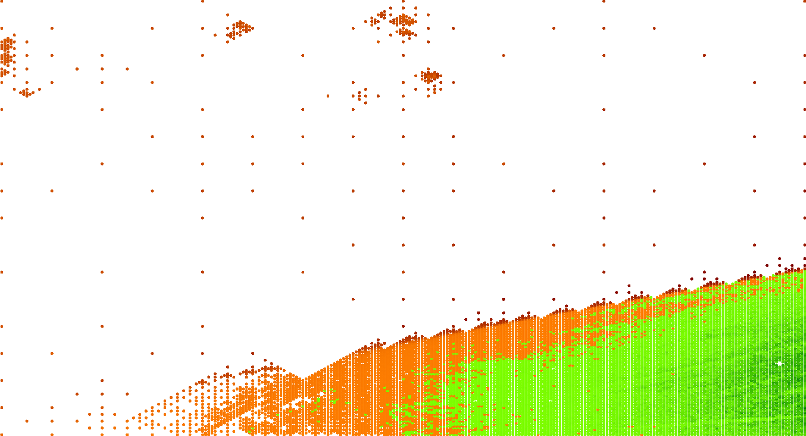
\includegraphics[width=0.9\textwidth]{1.0.0.Final/analysis1.png}}
	\end{subfigure}
	\begin{subfigure}[b]{0.3\textwidth}
		\fbox{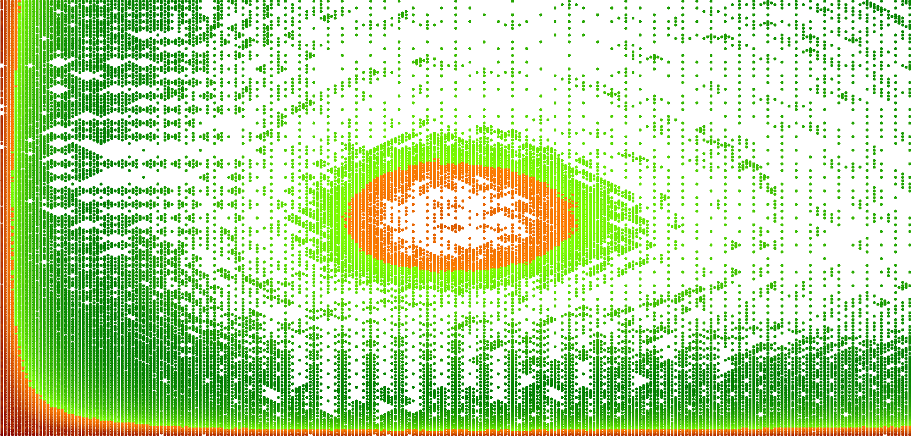
\includegraphics[width=0.9\textwidth]{1.0.0.Final/analysis2.png}}
		\centering
	\end{subfigure}
	\begin{subfigure}[b]{0.3\textwidth}
		\centering
		\fbox{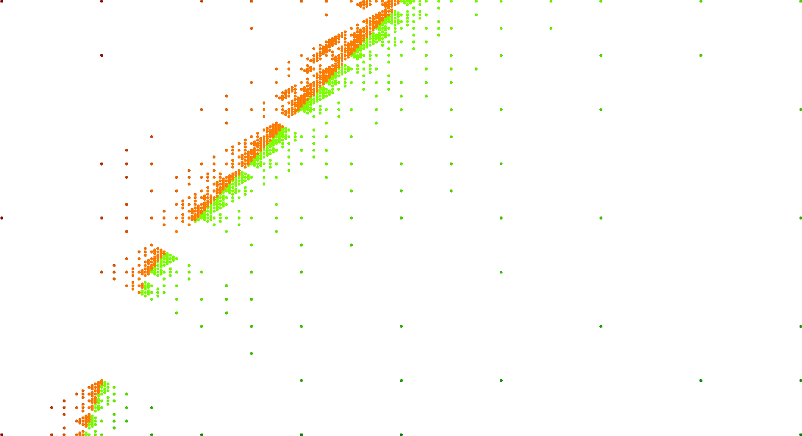
\includegraphics[width=0.9\textwidth]{1.0.0.Final/analysis3.png}}
	\end{subfigure}
	\caption{Ukázka vizualizace výsledku analýzy několika modelů. Zelené body označují hodnoty, kde daná vlastnost platí, v červených bodech vlastnost naopak neplatí.}
	\label{fig:vizualizace}
\end{figure}

\section{Čtvrtá etapa}

Ve čtvrté etapě, probíhající od začátku do konce listopadu, jsme pracovali na dokončení grafického rozhraní a
optimalizaci výpočtu, který se již v této etapě prováděl paralelně. Z hlediska optimalizace šlo zejména o:

\begin{itemize}
	\item	odstranění duplicitních výpočtů, zejména zlepšíním práce cache, ve které se ukládají již odsimulované trajektorie,
	\item	odstranění referencí na data již nepotřebných odsimulovaných trajektorií, aby mohla být zpracována pomocí \textit{garbage collectoru}.
\end{itemize}

Grafické rozhraní bylo do konce čtvrté etapy uvedeno do zcela funkčního stavu (viz \figurename\,\ref{fig:gui}). Komponenta zobrazující výsledky analýzy
byla upravena tak, aby po kliknutí na bod výsledku odsimulovala příslušnou trajektorii, což se ukázalo jako nutné v~průběhu třetí fáze (viz minulý report\footnote{
\url{https://github.com/sybila/parasim/blob/master/docs/reports/1.0.0.M2-3.pdf?raw=true}}). Tato funkce byla naimplementována jednodušším způsobem, než se původně plánovalo,
což však umožnilo přesunout práci na manažer pro správu projektů. Přitom je její současná podoba zcela dostačující. Zároveň bylo grafické rozhraní rozšířeno o~komponentu
zobrazující stav analýzy, což významnou měrou přispívá k~interaktivitě aplikace.

Vydaná verze z~konce čtvrté etapy je k~dispozici na stránkách našeho projektu\footnote{\url{https://github.com/sybila/parasim/zipball/1.0.0.M4}},
kde najdete též seznam vyřešených úkolů\footnote{\url{https://github.com/sybila/parasim/issues?milestone=6&state=closed}}.

\section{Pátá etapa}

V páté etapě, probíhající od začátku do konce prosince, jsme pracovali na vydání finální verze aplikace, psaní testů a dokumentace\footnote{\url{https://github.com/sybila/parasim/wiki}},
včetně tutorialu s~obrázky. Dále jsme se zaměřili na: 

\begin{itemize}
	\item	spuštění analýzy nad dalšími reálnými modely (viz \figurename\,\ref{fig:vizualizace}),
	\item	přidání globální robustnosti do analýzy,
	\item	zjednodušení nastavení analýzy (bylo odstraněno nastavení pro počáteční rozdělení prostoru iniciálních hodnot).
\end{itemize}

\begin{figure}[h!]
	\centering
	\begin{subfigure}[b]{0.48\textwidth}
		\centering
		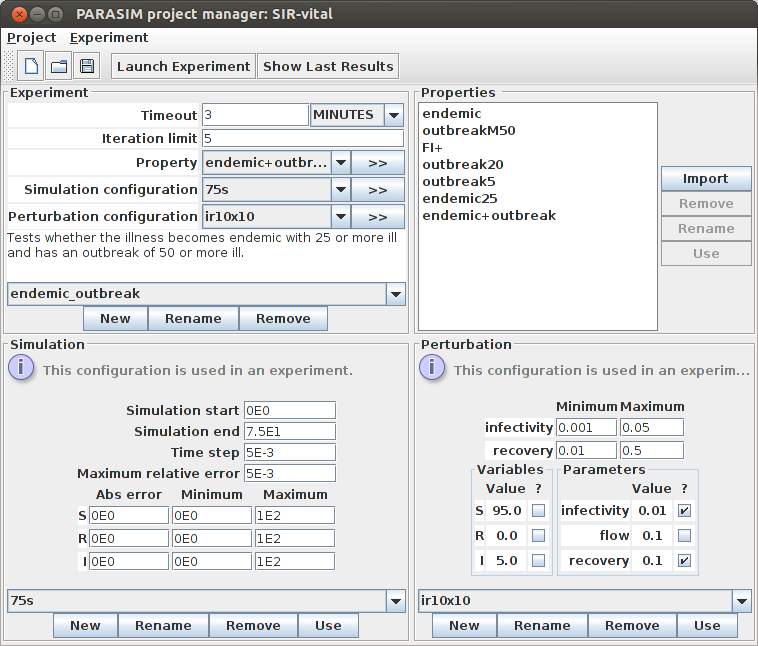
\includegraphics[width=0.8\textwidth]{1.0.0.Final/project-manager.png}
		\caption{Manažer pro správu.}
	\end{subfigure}
	\begin{subfigure}[b]{0.48\textwidth}
		\centering		
		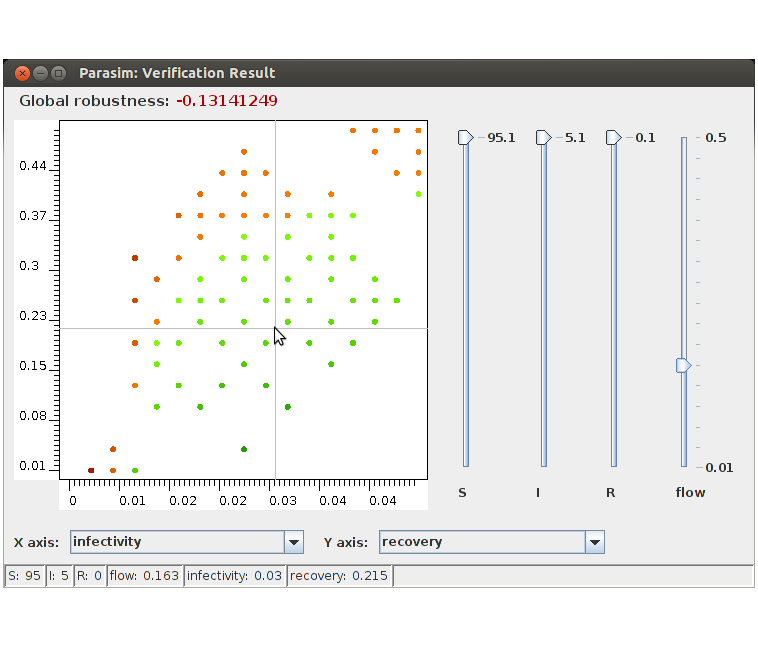
\includegraphics[width=0.8\textwidth]{1.0.0.Final/plotter.png}
		\caption{Komponenta pro vizualizaci výsledků analýzy.}
	\end{subfigure}
	\caption{Screenshoty z aplikace s grafickým rozhraním.}
	\label{fig:gui}
\end{figure}

Finální verze z konce páté etapy je k~dispozici na stránkách našeho projektu\footnote{\url{https://github.com/sybila/parasim/zipball/1.0.0.Final}},
kde najdete též seznam vyřešených úkolů\footnote{\url{https://github.com/sybila/parasim/issues?milestone=3&page=1&state=closed}}.

\section{Shrnutí}

Byl vytvořen nástroj pro analýzu dynamických systémů modelovaných pomocí
obyčejných diferenciálních rovnic. Tento nástroj je postaven na modulární architektuře,
která usnadňuje vstup třetí strany do vývoje nástroje. Možnost jednoduše zaměnit nové moduly
za ty stávající umožňuje optimalizaci a paralelizaci jednotlivých analytických algoritmů,
stejně jako zavádění úplně nových součástí nástroje.

Nástroj je tvořen dvěma aplikacemi: Grafickým rozhraním pro správu modelů, vlastností a nastavení analýzy
a aplikací spustitelnou z~příkazové řádky vhodnou zejména pro dávkové zpracování. Obě aplikace dokáží spustit
analýzu a zobrazit její výsledek a nastavení analýzy vytvořená v~grafickém rozrhaní dokáže přečíst i aplikace
z~příkazové řádky.

Repozitář projektu obsahuje několik reálných modelů s~přiloženými vlastnostmi a předpřipravenými analýzami,
nad kterými byl nástroj vyzkoušen. Kdokoliv si může analýzu nad těmito modely pustit sám, modely
a vlastnosti dále rozšiřovat, případně přidávat další.

Během řešení projektu se objevilo několik cest, kterými by se mohl ubírat další vývoj. Zejména se jedná o:

\begin{itemize}
	\item	vytvoření webovou službu zpřístupňující analýzu online,
	\item	použítí rychlejších nástrojů pro řešení obyčejných diferenciálních rovnic \footnote{momentálně je použit Octave, \url{http://octave.sourceforge.net/}},
	\item	zahrnutí projekce do vizualizace výsledků analýzy.
\end{itemize}

\end{document}

